\chapter{Aesthetic specifications}\label{cha:specifications}

This appendix summarises the various formats that \textbf{grid} drawing
functions take. Most of this information is available scattered
throughout the R documentation. This appendix brings it all together in
one place. \index{Aesthetics!specifications}

\section{Colour}\label{sec:colourux5fspec}

Colours can be specified with: \index{Colour!specifying}

\begin{itemize}
\itemsep1pt\parskip0pt\parsep0pt
\item
  A \textbf{name}, e.g., \texttt{"red"}. The colours are displayed in
  Figure \ref{fig:colours}, and can be listed in more detail with
  \texttt{colours()}. The Stowers Institute provides a nice printable
  pdf that lists all colours:
  \url{http://research.stowers-institute.org/efg/R/Color/Chart/}.
\item
  An \textbf{rgb specification}, with a string of the form
  \texttt{"\#RRGGBB"} where each of the pairs \texttt{RR}, \texttt{GG},
  \texttt{BB} consists of two hexadecimal digits giving a value in the
  range \texttt{00} to \texttt{FF}. Colors can be made partially
  transparent with \texttt{alpha}, e.g., \texttt{alpha = 0.5}.
\item
  An \textbf{NA}, for a completely transparent colour.
\end{itemize}

The functions \texttt{rgb()}, \texttt{hsv()}, \texttt{hcl()} can be used
to create colours specified in different colour spaces.

\section{Line type}\label{sec:line-type-spec}

Line types can be specified with: \index{Line type!specifying}

\begin{itemize}
\itemsep1pt\parskip0pt\parsep0pt
\item
  An \textbf{integer} or \textbf{name}: 0=blank, 1=solid, 2=dashed,
  3=dotted, 4=dotdash, 5=longdash, 6=twodash), illustrated in Figure
  \ref{fig:linetype}. *b The lengths of on/off stretches of line. This
  is done with a string of an even number (up to eight) of hexadecimal
  digits which give the lengths in consecutive positions in the string.
  For example, the string \texttt{"33"} specifies three units on
  followed by three off and \texttt{"3313"} specifies three units on
  followed by three off followed by one on and finally three off.
\end{itemize}

The five standard dash-dot line types described above correspond to 44,
13, 134, 73 and 2262.

Note that \texttt{NA} is not a valid value for \texttt{lty}.

\section{Shape}\label{sec:shape-spec}

Shapes take four types of values: \index{Shape!specifying}

\begin{itemize}
\itemsep1pt\parskip0pt\parsep0pt
\item
  An \textbf{integer} in \([0, 25]\), illustrated in Figure
  \ref{fig:shape}.
\item
  A \textbf{single character}, to use that character as a plotting
  symbol.\\
\item
  A \texttt{.} to draw the smallest rectangle that is visible (i.e.,
  about one pixel).
\item
  An \texttt{NA}, to draw nothing.
\end{itemize}

While all symbols have a foreground colour, symbols 19--25 also take a
background colour (fill).

\section{Size}\label{sec:size}

Throughout \texttt{ggplot}, for text height, point size and line width,
size is specified in millimetres. \index{Size!specifying}

\section{Justification}\label{sec:justification-spec}

Justification of a string (or legend) defines the location within the
string that is placed at the given position. There are two values for
horizontal and vertical justification. The values can be:
\index{Text justification} \indexc{hjust} \indexc{vjust}

\begin{itemize}
\itemsep1pt\parskip0pt\parsep0pt
\item
  A \textbf{string}: \texttt{"left"}, \texttt{"right"},
  \texttt{"centre"}, \texttt{"center"}, \texttt{"bottom"}, and
  \texttt{"top"}.
\item
  A \textbf{number} between 0 and 1, giving the position within the
  string (from bottom-left corner). These values are demonstrated in
  Figure \ref{fig:justification}.
\end{itemize}

\begin{Shaded}
\begin{Highlighting}[]
\CommentTok{# This code should recreate the figures, but we can't do fancy subfigures with knitr :(}
\KeywordTok{library}\NormalTok{(grid)}
\NormalTok{xquiet <-}\StringTok{ }\KeywordTok{scale_x_continuous}\NormalTok{(}\StringTok{""}\NormalTok{, }\DataTypeTok{breaks =} \OtherTok{NA}\NormalTok{)}
\NormalTok{yquiet <-}\StringTok{ }\KeywordTok{scale_y_continuous}\NormalTok{(}\StringTok{""}\NormalTok{, }\DataTypeTok{breaks =} \OtherTok{NA}\NormalTok{)}
\NormalTok{fill <-}\StringTok{ }\KeywordTok{theme}\NormalTok{(}
  \DataTypeTok{plot.margin =} \KeywordTok{unit}\NormalTok{(}\KeywordTok{rep}\NormalTok{(}\DecValTok{0}\NormalTok{, }\DecValTok{4}\NormalTok{), }\StringTok{"cm"}\NormalTok{), }
  \DataTypeTok{axis.text.x =} \KeywordTok{element_blank}\NormalTok{(),}
  \DataTypeTok{axis.text.y =} \KeywordTok{element_blank}\NormalTok{(),}
  \DataTypeTok{axis.title.x =} \KeywordTok{element_blank}\NormalTok{(),}
  \DataTypeTok{axis.title.y =} \KeywordTok{element_blank}\NormalTok{(),}
  \DataTypeTok{axis.ticks.length =} \KeywordTok{unit}\NormalTok{(}\DecValTok{0}\NormalTok{, }\StringTok{"cm"}\NormalTok{),}
  \DataTypeTok{axis.ticks.margin =} \KeywordTok{unit}\NormalTok{(}\DecValTok{0}\NormalTok{, }\StringTok{"cm"}\NormalTok{),}
  \DataTypeTok{panel.grid.major =} \KeywordTok{element_blank}\NormalTok{(),}
  \DataTypeTok{panel.grid.minor =} \KeywordTok{element_blank}\NormalTok{(),}
  \DataTypeTok{plot.background =} \KeywordTok{element_rect}\NormalTok{(}\DataTypeTok{fill =} \StringTok{"grey90"}\NormalTok{, }\DataTypeTok{colour =} \OtherTok{NA}\NormalTok{)}
\NormalTok{)}

\CommentTok{# Shapes ---------------------------------------------------------}
\NormalTok{shapes <-}\StringTok{ }\KeywordTok{data.frame}\NormalTok{(}
  \DataTypeTok{shape =} \KeywordTok{c}\NormalTok{(}\DecValTok{0}\NormalTok{:}\DecValTok{19}\NormalTok{, }\DecValTok{22}\NormalTok{, }\DecValTok{21}\NormalTok{, }\DecValTok{24}\NormalTok{, }\DecValTok{23}\NormalTok{, }\DecValTok{20}\NormalTok{),}
  \DataTypeTok{x =} \DecValTok{0}\NormalTok{:}\DecValTok{24} \NormalTok\StringTok{ }\DecValTok{5}\NormalTok{,}
  \DataTypeTok{y =} \NormalTok{-(}\DecValTok{0}\NormalTok{:}\DecValTok{24} \NormalTok\StringTok{ }\DecValTok{5}\NormalTok{)}
\NormalTok{)}
\KeywordTok{qplot}\NormalTok{(x, y, }\DataTypeTok{data=}\NormalTok{shapes, }\DataTypeTok{shape=}\NormalTok{shape, }\DataTypeTok{size=}\KeywordTok{I}\NormalTok{(}\DecValTok{5}\NormalTok{), }\DataTypeTok{fill=}\KeywordTok{I}\NormalTok{(}\StringTok{"blue"}\NormalTok{)) +}
\StringTok{  }\KeywordTok{scale_shape_identity}\NormalTok{() +}\StringTok{ }\KeywordTok{xlim}\NormalTok{(}\DecValTok{0}\NormalTok{, }\FloatTok{4.4}\NormalTok{) +}\StringTok{ }
\StringTok{  }\KeywordTok{geom_text}\NormalTok{(}\KeywordTok{aes}\NormalTok{(}\DataTypeTok{x =} \NormalTok{x +}\StringTok{ }\FloatTok{0.2}\NormalTok{, }\DataTypeTok{label=}\NormalTok{shape), }\DataTypeTok{hjust=}\DecValTok{0}\NormalTok{) +}\StringTok{ }\NormalTok{fill}

\CommentTok{# Line types -----------------------------------------------------------------}
\NormalTok{lty <-}\StringTok{ }\KeywordTok{c}\NormalTok{(}\StringTok{"blank"}\NormalTok{, }\StringTok{"solid"}\NormalTok{, }\StringTok{"dashed"}\NormalTok{, }\StringTok{"dotted"}\NormalTok{, }\StringTok{"dotdash"}\NormalTok{, }
         \StringTok{"longdash"}\NormalTok{,}\StringTok{"twodash"}\NormalTok{)}
\NormalTok{linetypes <-}\StringTok{ }\KeywordTok{data.frame}\NormalTok{(}
  \DataTypeTok{y =} \KeywordTok{seq_along}\NormalTok{(lty),}
  \DataTypeTok{lty =} \NormalTok{lty}
\NormalTok{) }
\KeywordTok{qplot}\NormalTok{(}\DecValTok{0}\NormalTok{, y, }\DataTypeTok{data=}\NormalTok{linetypes, }\DataTypeTok{xend =} \DecValTok{5}\NormalTok{, }\DataTypeTok{yend=}\NormalTok{y, }\DataTypeTok{geom=}\StringTok{"segment"}\NormalTok{, }\DataTypeTok{linetype=}\NormalTok{lty) +}
\StringTok{  }\KeywordTok{scale_linetype_identity}\NormalTok{() +}\StringTok{ }
\StringTok{  }\KeywordTok{geom_text}\NormalTok{(}\KeywordTok{aes}\NormalTok{(}\DataTypeTok{x =} \DecValTok{0}\NormalTok{, }\DataTypeTok{y =} \NormalTok{y +}\StringTok{ }\FloatTok{0.2}\NormalTok{, }\DataTypeTok{label =} \NormalTok{lty), }\DataTypeTok{hjust =} \DecValTok{0}\NormalTok{) +}\StringTok{ }
\StringTok{  }\NormalTok{fill}

\CommentTok{# Justification --------------------------------------------------------------}

\NormalTok{draw.text <-}\StringTok{ }\NormalTok{function(just, i, j) \{}
 \KeywordTok{grid.text}\NormalTok{(}\StringTok{"ABCD"}\NormalTok{, }\DataTypeTok{x=}\NormalTok{x[j], }\DataTypeTok{y=}\NormalTok{y[i], }\DataTypeTok{just=}\NormalTok{just, }\DataTypeTok{gp=}\KeywordTok{gpar}\NormalTok{(}\DataTypeTok{fontsize=}\DecValTok{16}\NormalTok{, }\DataTypeTok{colour =}\StringTok{"black"}\NormalTok{))}
 \KeywordTok{grid.text}\NormalTok{(}\KeywordTok{deparse}\NormalTok{(}\KeywordTok{substitute}\NormalTok{(just)), }\DataTypeTok{x=}\NormalTok{x[j], }\DataTypeTok{y=}\NormalTok{y[i] +}\StringTok{ }\KeywordTok{unit}\NormalTok{(}\DecValTok{2}\NormalTok{, }\StringTok{"lines"}\NormalTok{),}
           \DataTypeTok{gp=}\KeywordTok{gpar}\NormalTok{(}\DataTypeTok{col=}\StringTok{"grey30"}\NormalTok{, }\DataTypeTok{fontsize=}\DecValTok{8}\NormalTok{, }\DataTypeTok{fontface=}\StringTok{"bold"}\NormalTok{))}
\NormalTok{\}}

\KeywordTok{grid.newpage}\NormalTok{()}
\KeywordTok{grid.rect}\NormalTok{(}\DataTypeTok{gp=} \KeywordTok{gpar}\NormalTok{(}\DataTypeTok{fill=}\StringTok{"grey90"}\NormalTok{, }\DataTypeTok{col=}\OtherTok{NA}\NormalTok{))}
\NormalTok{pos <-}\StringTok{ }\KeywordTok{c}\NormalTok{(}\FloatTok{0.2}\NormalTok{, }\FloatTok{0.5}\NormalTok{, }\FloatTok{0.8}\NormalTok{)}
\NormalTok{x <-}\StringTok{ }\KeywordTok{unit}\NormalTok{(pos, }\StringTok{"npc"}\NormalTok{)}
\NormalTok{y <-}\StringTok{ }\KeywordTok{unit}\NormalTok{(pos, }\StringTok{"npc"}\NormalTok{)}
\KeywordTok{grid.grill}\NormalTok{(}\DataTypeTok{h=}\NormalTok{y, }\DataTypeTok{v=}\NormalTok{x, }\DataTypeTok{gp=}\KeywordTok{gpar}\NormalTok{(}\DataTypeTok{col=}\StringTok{"white"}\NormalTok{))}
\KeywordTok{draw.text}\NormalTok{(}\KeywordTok{c}\NormalTok{(}\DecValTok{0}\NormalTok{,   }\DecValTok{0}\NormalTok{), }\DecValTok{1}\NormalTok{, }\DecValTok{1}\NormalTok{)}
\KeywordTok{draw.text}\NormalTok{(}\KeywordTok{c}\NormalTok{(}\FloatTok{0.5}\NormalTok{, }\DecValTok{0}\NormalTok{), }\DecValTok{2}\NormalTok{, }\DecValTok{1}\NormalTok{)}
\KeywordTok{draw.text}\NormalTok{(}\KeywordTok{c}\NormalTok{(}\DecValTok{1}\NormalTok{,   }\DecValTok{0}\NormalTok{), }\DecValTok{3}\NormalTok{, }\DecValTok{1}\NormalTok{)}

\KeywordTok{draw.text}\NormalTok{(}\KeywordTok{c}\NormalTok{(}\DecValTok{0}\NormalTok{,   }\FloatTok{0.5}\NormalTok{), }\DecValTok{1}\NormalTok{, }\DecValTok{2}\NormalTok{)}
\KeywordTok{draw.text}\NormalTok{(}\KeywordTok{c}\NormalTok{(}\FloatTok{0.5}\NormalTok{, }\FloatTok{0.5}\NormalTok{), }\DecValTok{2}\NormalTok{, }\DecValTok{2}\NormalTok{)}
\KeywordTok{draw.text}\NormalTok{(}\KeywordTok{c}\NormalTok{(}\DecValTok{1}\NormalTok{,   }\FloatTok{0.5}\NormalTok{), }\DecValTok{3}\NormalTok{, }\DecValTok{2}\NormalTok{)}

\KeywordTok{draw.text}\NormalTok{(}\KeywordTok{c}\NormalTok{(}\DecValTok{0}\NormalTok{,   }\DecValTok{1}\NormalTok{), }\DecValTok{1}\NormalTok{, }\DecValTok{3}\NormalTok{)}
\KeywordTok{draw.text}\NormalTok{(}\KeywordTok{c}\NormalTok{(}\FloatTok{0.5}\NormalTok{, }\DecValTok{1}\NormalTok{), }\DecValTok{2}\NormalTok{, }\DecValTok{3}\NormalTok{)}
\KeywordTok{draw.text}\NormalTok{(}\KeywordTok{c}\NormalTok{(}\DecValTok{1}\NormalTok{,   }\DecValTok{1}\NormalTok{), }\DecValTok{3}\NormalTok{, }\DecValTok{3}\NormalTok{)}

\CommentTok{# Colour ---------------------------------------------------------------------}
\KeywordTok{source}\NormalTok{(}\StringTok{"colour-wheel.R"}\NormalTok{)}
\KeywordTok{qplot}\NormalTok{(x, y, }\DataTypeTok{data=}\NormalTok{hcl, }\DataTypeTok{colour=}\NormalTok{colour) +}\StringTok{ }
\StringTok{  }\KeywordTok{scale_colour_identity}\NormalTok{() +}\StringTok{ }
\StringTok{  }\KeywordTok{coord_equal}\NormalTok{() +}\StringTok{ }
\StringTok{  }\NormalTok{fill}
\end{Highlighting}
\end{Shaded}

\begin{figure}[htbp]
  \centering
  \subfigure[All named colours in Luv space]{
    \label{fig:colours}
    \includegraphics[width=0.45\linewidth]{diagrams/spec-colour}
  }
  \subfigure[Built-in line types]{
    \label{fig:linetype}
    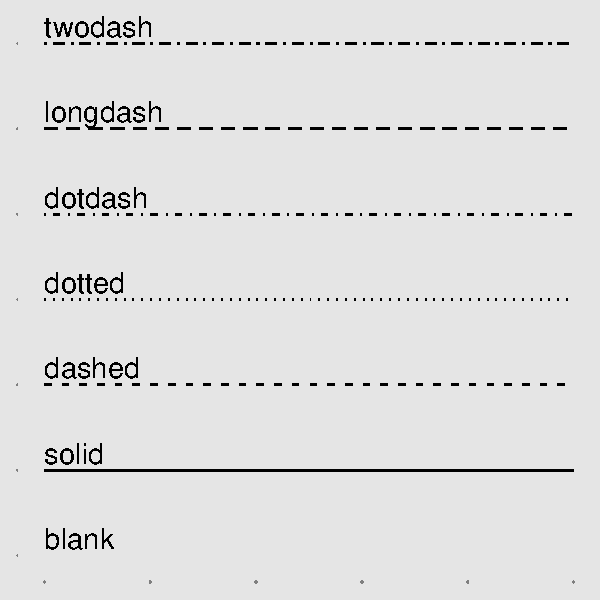
\includegraphics[width=0.45\linewidth]{diagrams/spec-linetype}
  }
  \subfigure[R plotting symbols.  Colour is black, and fill is blue.  Symbol 25 (not shown) is symbol 24 rotated 180 degrees.]{
    \label{fig:shape}
    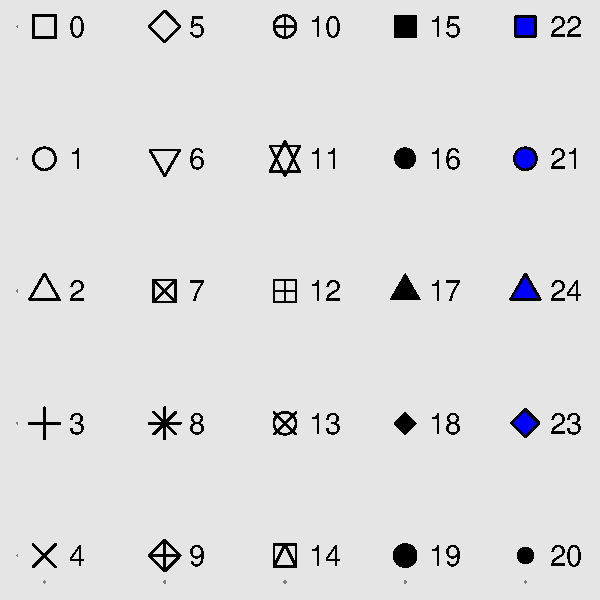
\includegraphics[width=0.45\linewidth]{diagrams/spec-shape}  
  }
  \subfigure[Horizontal and vertical justification settings.]{
    \label{fig:justification}
    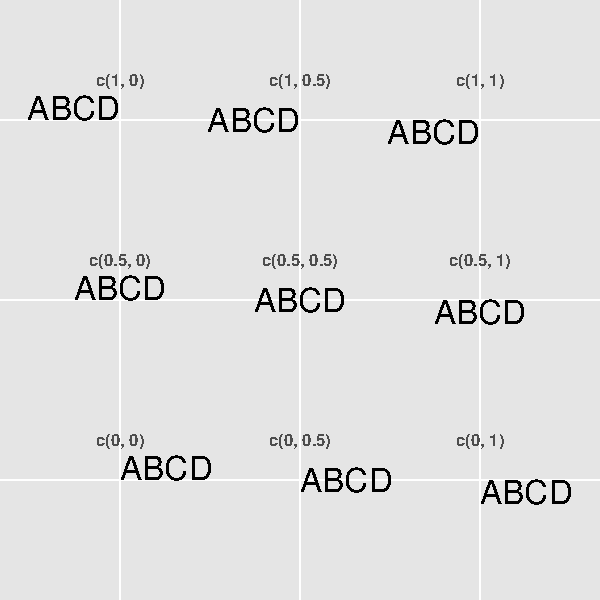
\includegraphics[width=0.45\linewidth]{diagrams/spec-justification}
  }
  \caption{Examples illustrating different aesthetic settings.}
\end{figure}
